\graphicspath{ {Figures/Pileup/Energies/} {Figures/Pileup/TimeSpectra/} {Figures/Main/} {Figures/ResidualsFFT/} {Figures/FitStartScans/} {Figures/PerCalo/} }

\chapter{Analysis Results}
\label{Ch:Results}

\section{Pre-corrected and corrected energy and time spectra}

	Before fitting the data and extracting the \gmtwo frequency, pileup has to be removed. The procedure to do this was detailed in Section \ref{Sec:PileupCorrection}, and the results are shown here. Figure \ref{fig:PileupTimeSpectrum} shows the constructed pileup time spectrum, for pileup energies above threshold. The pre-corrected and corrected time spectra are not shown because differences are small and hard to see. As shown the pileup is almost completely gone by $\SI{300}{\mu s}$. The exact shape of the pileup time spectra is explained in DocDB 14394, which is in general unimportant as long as it is constructed and subtracted properly. Figure \ref{fig:ClusterEnergiesVsPileupEnergies} shows a comparison between the cluster energies and the constructed pileup energies, where differences in the two spectra are small and can be attributed to pileup contamination in the shadow method and triplets which have not been included in this analysis. Figures \ref{fig:AddedEnergies}, \ref{fig:CaloEnergies}, and \ref{fig:CaloEnergiesZoomed} show the pre-corrected and corrected energy spectra for the added histograms and for some individual calorimeters. Since the pileup energies are not perfectly reconstructed the corrected energy spectrum does not converge to 0 at the end of the high energy tail, which is readily seen in the log-scale plots. This is okay for the level of statistics included in both the 60H dataset and in Run 1. Systematic effects from getting the pileup amplitude or shape wrong are explored in Section \ref{Sec:SystematicPileup}.

	\begin{figure}[]
		\centering
		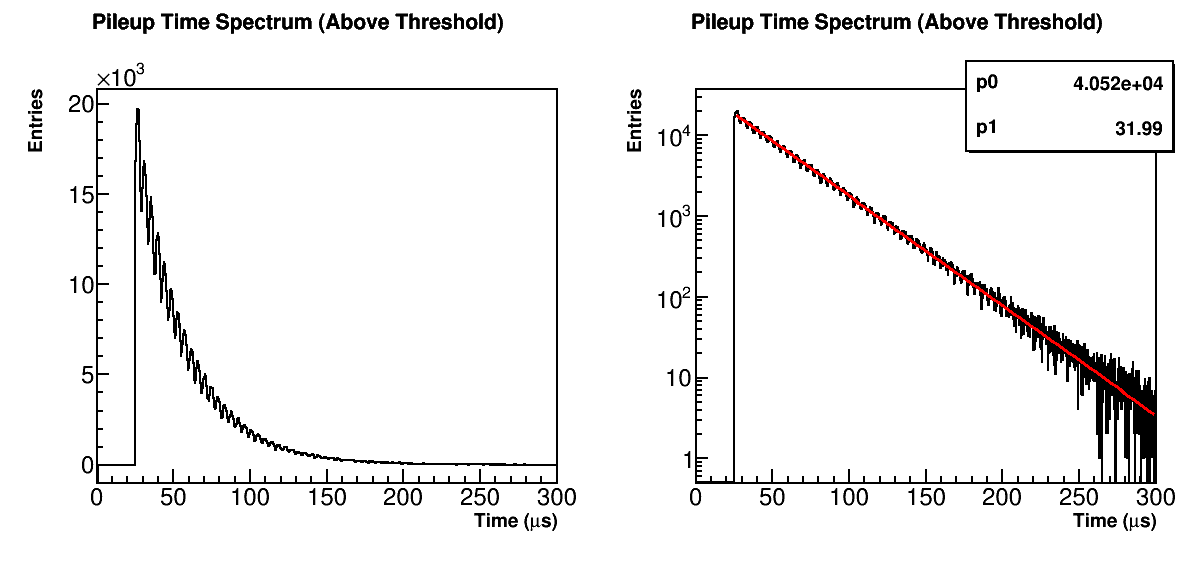
\includegraphics[width=\textwidth]{PileupTimeSpectrum}
	    \caption[PileupTimeSpectrum]{Plotted is constructed pileup time spectrum on a linear (left) and log (right) scale. The histogram on the right is fit to a simple two parameter exponential to get an idea of the lifetime of the pileup, calculated here as $\SI{32.02}{\mu s}$, which is close to half of the muon lifetime at about $\SI{64.4}{\mu s}$. Reasons for why these two values don't equal include the absence of triplets, lost muons, and an improper fitting function.}
	    \label{fig:PileupTimeSpectrum}
	\end{figure}

	\begin{figure}[]
		\centering
		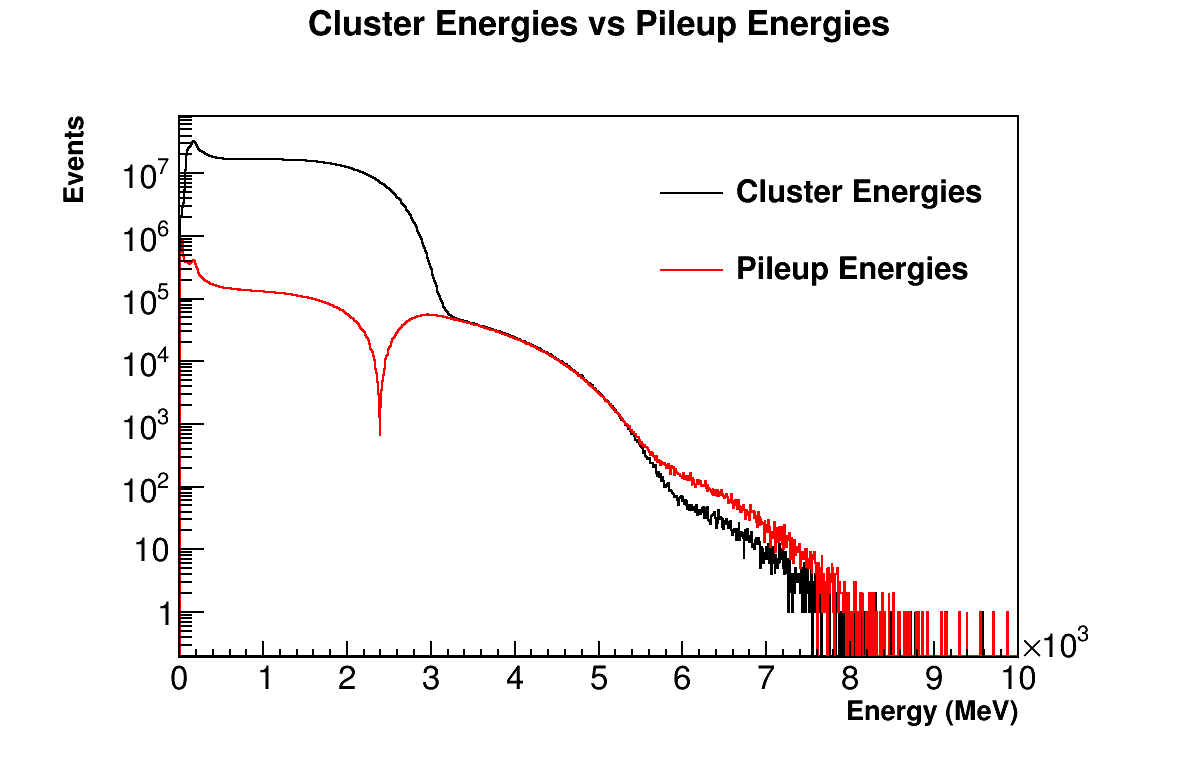
\includegraphics[width=\textwidth]{ClusterEnergiesVsPileupEnergies}
	    \caption[ClusterEnergiesVsPileupEnergies]{Cluster energies in black are plotted vs pileup energies in red, for all calorimeters added together. At energies below about 2.4 GeV the pileup spectrum goes negative. In this plot the absolute value of the pileup energies is plotted, and a spike at about 2.4 GeV can be seen as a consequence of this.}    
	    \label{fig:ClusterEnergiesVsPileupEnergies}
	\end{figure}

	\begin{figure}[]
	\centering
	    \begin{subfigure}[]{0.8\textwidth}
		    \centering
			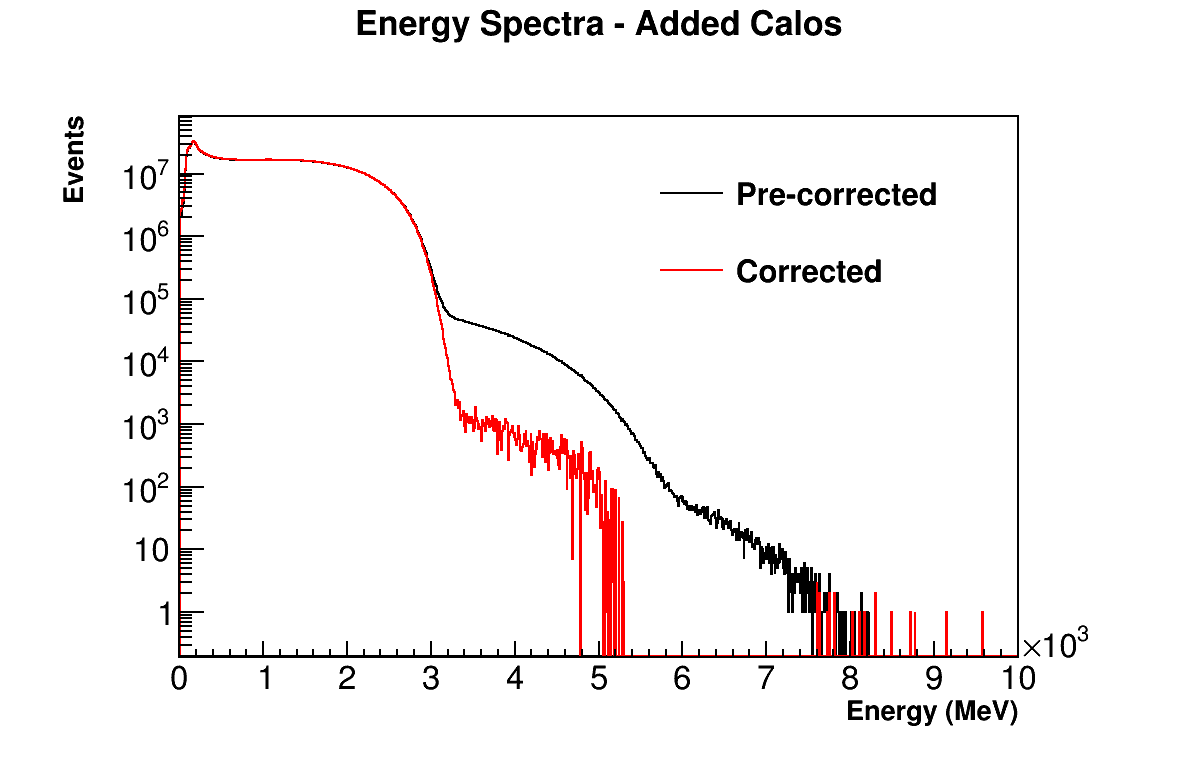
\includegraphics[width=\textwidth]{AddedEnergies}
		    \caption{Log scale - the corrected energy spectrum goes negative around 5 GeV.}
	    \end{subfigure}% %you need this % here to add spacing between subfigures
	    \vspace{1cm}
	    \begin{subfigure}[]{0.8\textwidth}
		    \centering
			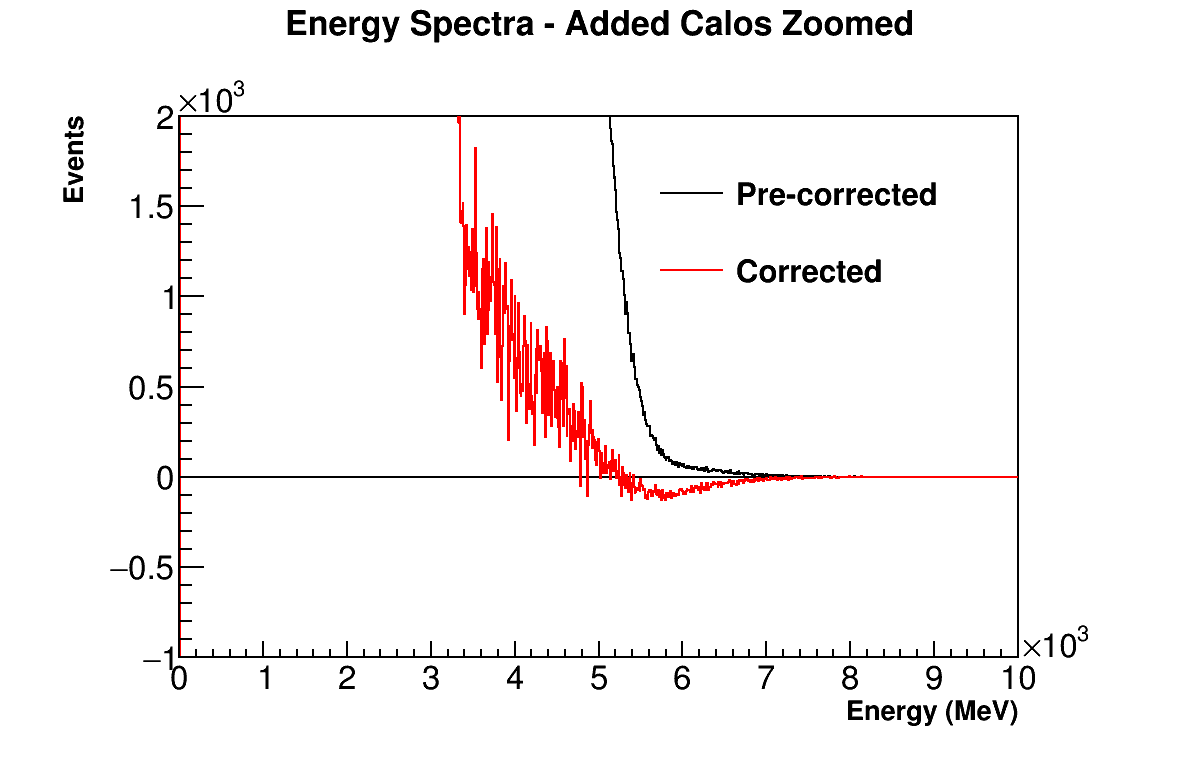
\includegraphics[width=\textwidth]{AddedEnergiesZoomed}
		    \caption{Linear scale - zoomed in to show the shape.}
	    \end{subfigure}
	\caption[AddedEnergies]{Plots for the pre-corrected and corrected energy spectra are shown, all calorimeters added together. Because the triplets and contamination are not accounted for, the corrected energy spectrum does not lie exacltly along zero.}
	\label{fig:AddedEnergies}
	\end{figure}

	\begin{figure}[]
		\centering
		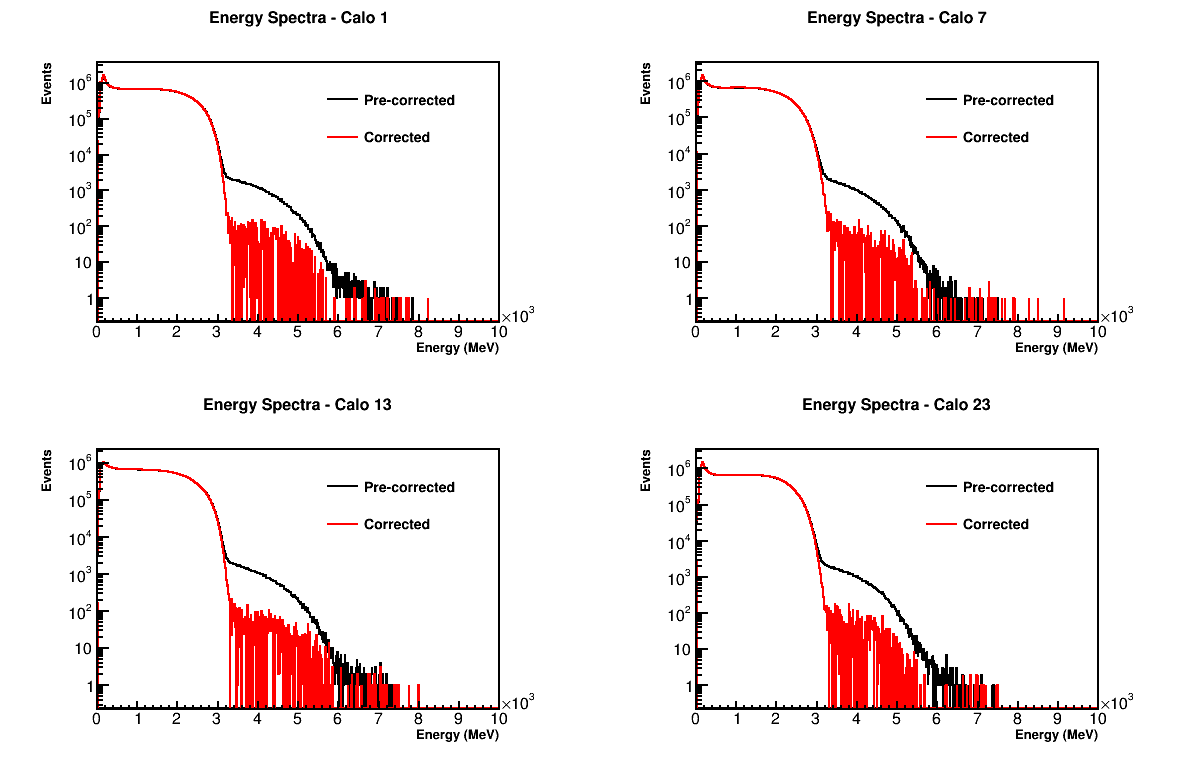
\includegraphics[width=.8\textwidth]{CaloEnergies}
	    \caption[CaloEnergies]{Pre-corrected and corrected energy spectra for calorimeters 1, 7, 13, and 23 plotted on a log scale.}    
	    \label{fig:CaloEnergies}
	\end{figure}

	\begin{figure}[]
		\centering
		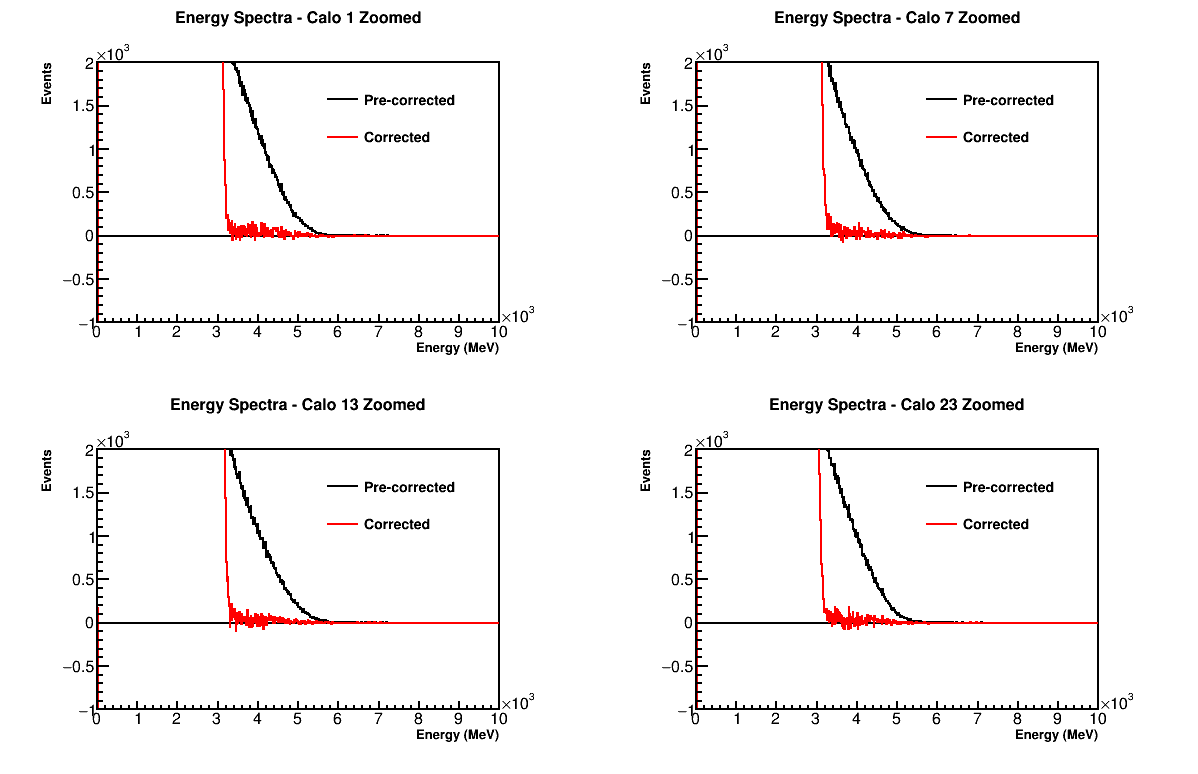
\includegraphics[width=.8\textwidth]{CaloEnergiesZoomed}
	    \caption[CaloEnergiesZoomed]{Pre-corrected and corrected energy spectra for calorimeters 1, 7, 13, and 23 plotted on a linear scale and zoomed in.}    
	    \label{fig:CaloEnergiesZoomed}
	\end{figure}

\clearpage

\section{7 Parameter Ratio Fit}

	The data has been fit to a 7 parameter function, as described in Section \ref{Sec:FinalFitFunction}, reduced from the conventional 14 parameters in a T Method fit. The results are shown in Figure \ref{fig:ratioCBO_moduloPlot}, with the fit parameters transcribed into Table \ref{Tab:FitParams}. These 7 parameters include the asymmetry ``A'', the ppm level shift in the \gmtwo frequency ``R'', the \gmtwo phase ``$\phi$'', and then 4 CBO parameters. As detailed in Section \ref{Sec:CBO}, these CBO parameters include the frequency ``$\omega_{cbo}$'', lifetime ``$\tau_{cbo}$'', and then the CBO amplitude and phase on the N term, ``$N_{cbo-A}$'' and ``$N_{cbo-\phi}$'' respectively. The CBO lifetime has been fixed in the fit to $\SI{180}{\mu s}$. The N and muon lifetime terms are unecessary because the ratio method removes those terms in the data to be fit. The ratio method also divides out slow effects, which removes the need to fit for muon losses. The lack of a low frequency rise in the FFTs of the residuals as shown in Figure \ref{fig:FFT_ratioCBOFit} justifies excluding this term. Finally, due to the specific n value used in gathering the 60H data, the vertical waist (VW) frequency just so happens to be very nearly 10 times the \gmtwo frequency. As described in Section \ref{Sec:VW} this means that the VW does not need to be included in the fit. Like the lost muons this is justified by the lack of a VW peak in the FFT of the residuals. Finally, the fit range is restricted from $\SI{30}{\mu s} - \SI{500}{\mu s}$. The early time cut is determined due the instability of the stored muon beam at early times. The late time cut was chosen to avoid the region where the ratio actually starts to widen due to low stats. (This can actually be extended beyond $\SI{500}{\mu s}$ safely but that was the limit used by default for previous datasets, and was left in when analyzing the 60H dataset.)

	Table \ref{Tab:CorrMat} shows the correlation matrix for the fit parameters in the added calorimeter fit. Figure \ref{fig:CorrelationMatrix} shows the same information in graphical format. As seen the only significant correlation to R is the \gmtwo phase. This is good because it means that if other fit parameters are for some reason fitted slightly incorrectly, the resulting effect on R will be minimal.

	\begin{figure}[]
		\centering
		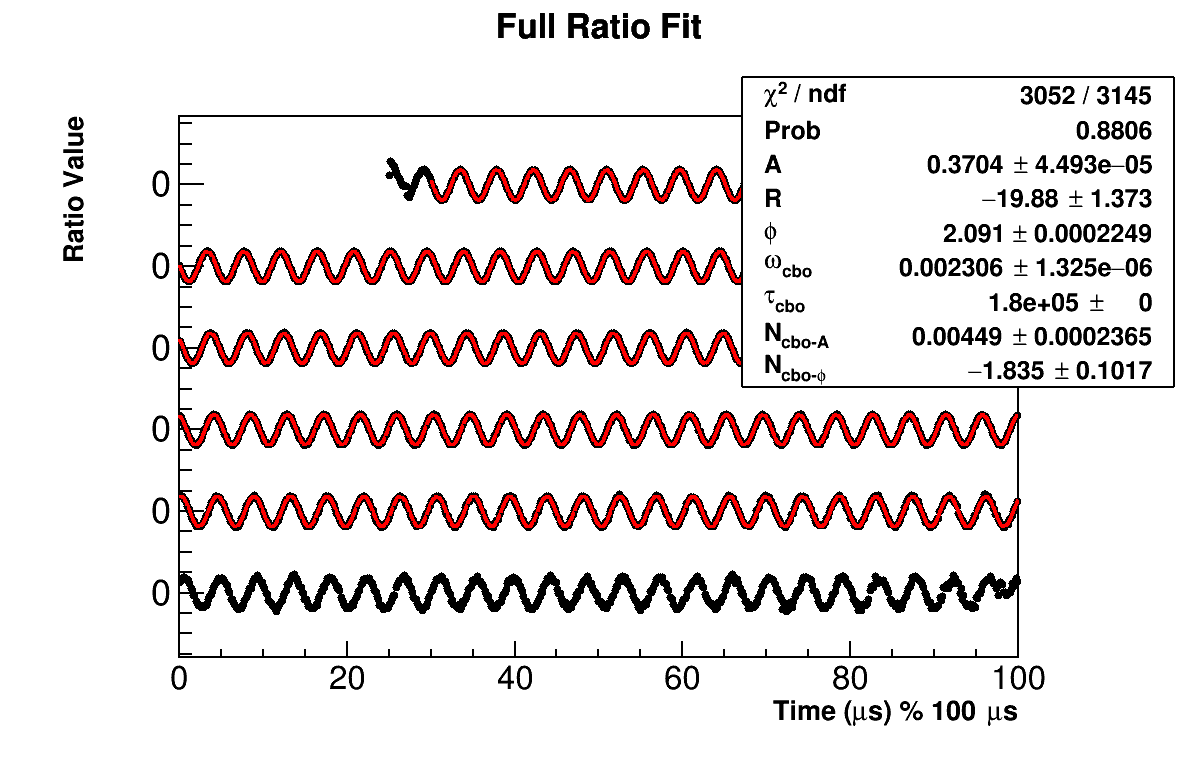
\includegraphics[width=\textwidth]{ratioCBO_moduloPlot}
	    \caption[ratioCBO_moduloPlot]{Final fit result for the 60 hour dataset. The fit includes 6 free parameters and one fixed. The x axis is in units of $\mu$s modulo 100 $\mu$s, with successive portions of the data points and fit shifted downwards on the plot. The parameter values in the stats box for the CBO frequency and lifetime are in units of ns. R is blinded locally. The fit ranges from 30 $\mu$s to 500 $\mu$s.}
	    \label{fig:ratioCBO_moduloPlot}
	\end{figure}

	\begin{table}[]
	\centering
	\setlength\tabcolsep{10pt}
	\renewcommand{\arraystretch}{1.2}
	\begin{tabular*}{.8\linewidth}{@{\extracolsep{\fill}}|l|l|c|c|}
	  \hline
	  	\multicolumn{4}{|c|}{\textbf{Fit Results}} \\
	  \hline\hline
	  	\multicolumn{2}{|c}{$\chi^{2}$/NDF}       				&  \multicolumn{2}{c|}{$3052/3145$}  \\
	  	\multicolumn{2}{|c}{P value}         	 				&  \multicolumn{2}{c|}{$0.8806$}  \\
	  \hline\hline
	  	Parameter & Descriptor & Value & Error \\
	  \hline
		$A$    			 	  & Asymmetry  	    			&  $0.3704$  	&	$\SI{4.493e-5}{}$  \\
		$R$     			  & R (ppm, blinded)   	 		&  $-19.88$  	&	$1.373$  \\
		$\phi$   			  & \gmtwo Phase         		&  $2.091$  	&	$\SI{2.249e-4}{}$  \\
		$\omega_{cbo}$   	  & CBO Frequency $(ns^{-1})$   &  $0.002306$  	&	$\SI{1.325e-6}{}$  \\
		$\tau_{cbo}$ (fixed)  & CBO Lifetime $(\mu s)$ 	    &  $180$  		&	$0$  \\
		$N_{cbo-A}$   	 	  & CBO N Amplitude      		&  $0.00449$  	&	$\SI{2.365e-4}{}$  \\
		$N_{cbo-\phi}$   	  & CBO N Phase       	 		&  $-1.835$  	&	$0.1017$  \\
	  \hline
	\end{tabular*}
	\caption{Table of final fit results.}
	\label{Tab:FitParams}
	\end{table}

	\begin{table}[]
	\setlength\tabcolsep{0pt}
	\begin{tabular*}{\linewidth}{@{\extracolsep{\fill}}lLBLLLLL}
	  \toprule
	            & \thead{$A$} & \thead{$R$} & \thead{$\phi$} & \thead{$\omega_{cbo}$} & \thead{$\tau_{cbo}$ (fixed)} & \thead{$N_{cbo-A}$} & \thead{$N_{cbo-\phi}$} \\
	  \midrule
		$A$    			 	 &  1.0000  &  0.0049  & -0.0068  & -0.0166  &  0.0000  & -0.0098  &  0.0233  \\
		$R$     			 &  0.0049  &  1.0000  & -0.8300  & -0.0204  &  0.0000  &  0.0207  &  0.0282  \\
		$\phi$   			 & -0.0068  & -0.8300  &  1.0000  &  0.0280  &  0.0000  & -0.0287  & -0.0387  \\
		$\omega_{cbo}$   	 & -0.0166  & -0.0204  &  0.0280  &  1.0000  &  0.0000  &  0.0773  & -0.8585  \\
		$\tau_{cbo}$ (fixed) &  0.0000  &  0.0000  &  0.0000  &  0.0000  &  1.0000  &  0.0000  &  0.0000  \\
		$N_{cbo-A}$   	 	 & -0.0098  &  0.0207  & -0.0287  &  0.0773  &  0.0000  &  1.0000  & -0.0656  \\
		$N_{cbo-\phi}$   	 &  0.0233  &  0.0282  & -0.0387  & -0.8585  &  0.0000  & -0.0656  &  1.0000  \\
	  \bottomrule
	\end{tabular*}
	\caption{Correlation matrix for the full ratio fit. The CBO lifetime is fixed but included in this table. The only significant correlation to R is the \gmtwo phase.}
	\label{Tab:CorrMat}
	\end{table}

	\begin{figure}[]
		\centering
		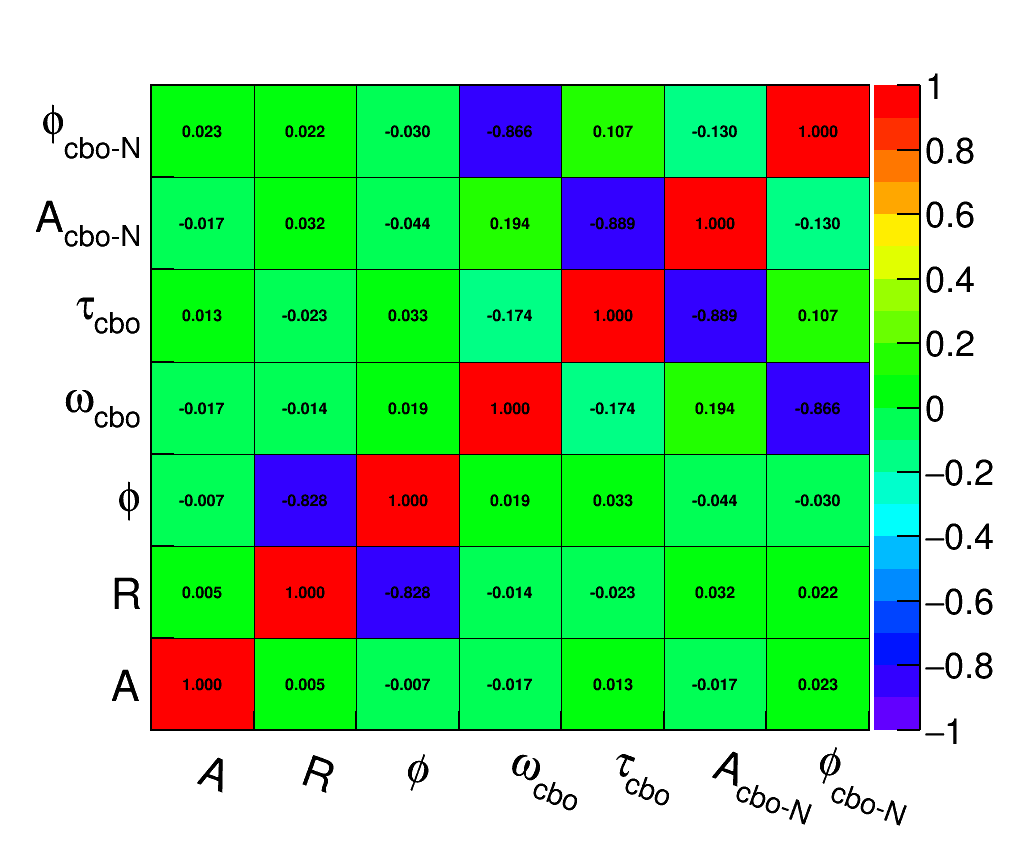
\includegraphics[width=\textwidth]{CorrelationMatrix}
	    \caption[CorrelationMatrix]{Plotted are the correlations between the different fit parameters. Correlations to R are minimal for all fit parameters except the \gmtwo phase. The correlation between the CBO frequency and phase is also easily noticed in this plot.}
	    \label{fig:CorrelationMatrix}
	\end{figure}

\clearpage

\section{Residual and FFT}

	In order to examine the goodness-of-fit, the residuals and the FFT of the residuals need to be examined. The residuals as well as the pulls are shown in Figure \ref{fig:fitResidual}. Also included is a plot of the pulls projected down onto the Y axis. In all three plots no substructure is immediately obvious, and in the latter the pull plot can be seen to have a mean consistent with 0 and an RMS consistent with 1, preliminarily indicating that the fit is good. Plotted in Figure \ref{fig:FFT_ratioCBOFit} is the FFT of the residuals. As can be seen no physical frequencies are observable above the noise. This shows that the CBO has been fitted correctly, and justifies the lack of a muon losses or vertical waist term in the fit. Figure \ref{fig:FFTComparison_RatioCBO} shows a similar plot, but this time overlayed with the FFT of the fit residuals for a 5 parameter fit. As seen the CBO, VW, \gmtwo, and their beat frequencies, as well as the lost muon peak at low frequencies are removed when performing the full ratio fit.


	\begin{figure}[h]
	\centering
	    \begin{subfigure}[]{0.45\textwidth}
		    \centering
			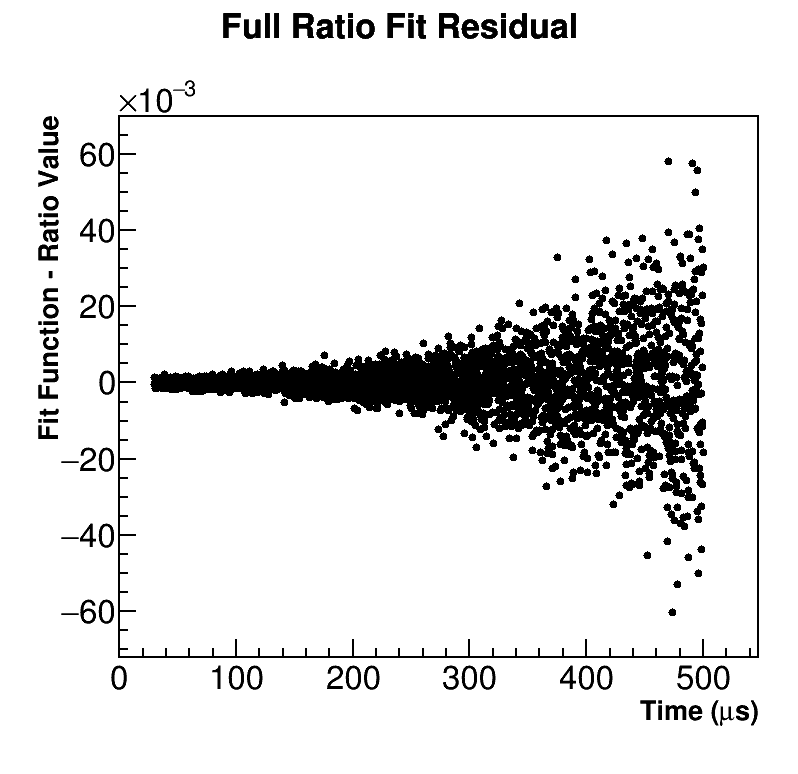
\includegraphics[width=\textwidth]{fitResidual}
		    \caption{Fit residuals.}
	    \end{subfigure}
	    \begin{subfigure}[]{0.45\textwidth}
		    \centering
			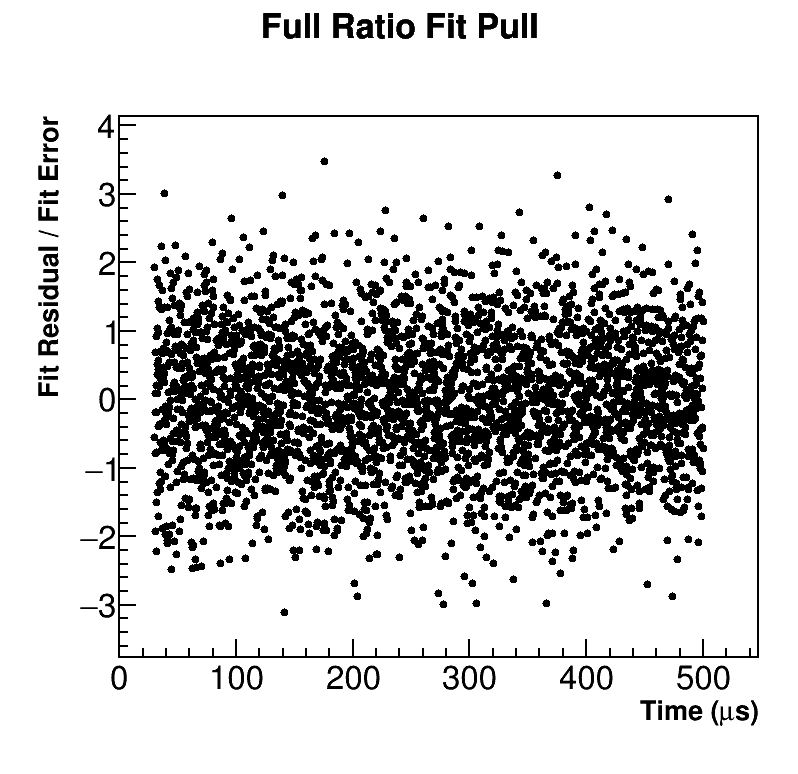
\includegraphics[width=\textwidth]{fitPull}
		    \caption{Fit pulls.}
	    \end{subfigure}% %you need this % here to add spacing between subfigures
	    \vspace{4mm}
	    \begin{subfigure}[]{0.7\textwidth}
		    \centering
			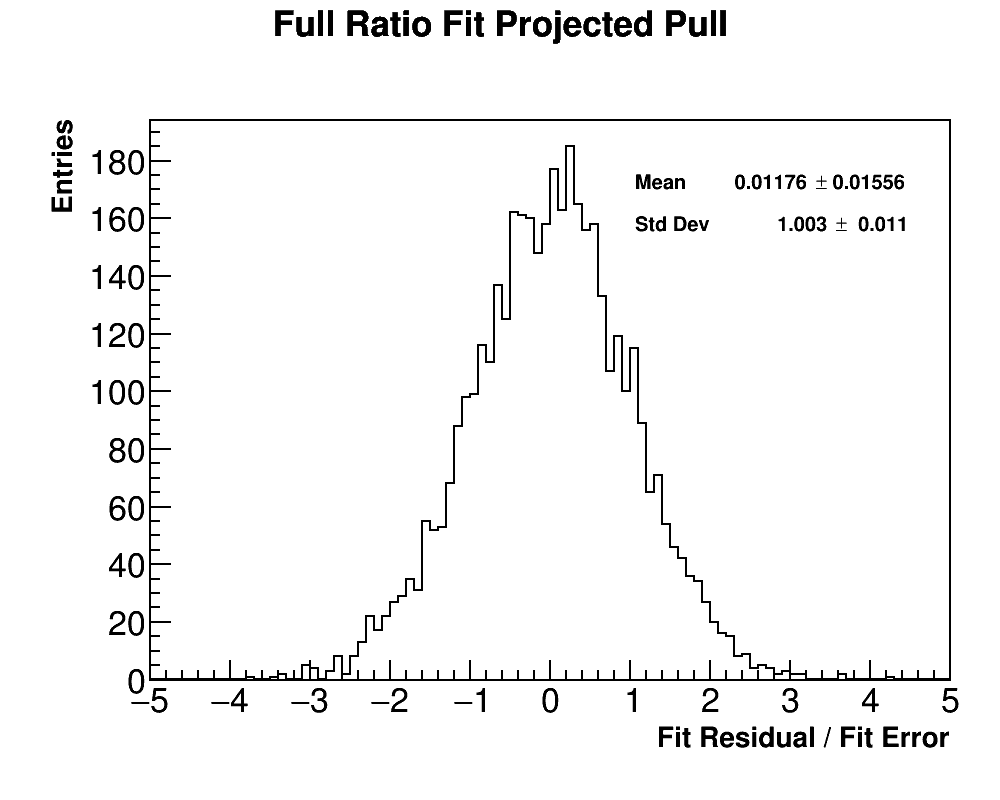
\includegraphics[width=\textwidth]{fitPull_projected}
		    \caption{Fit pulls projected onto the y axis. Note the Gaussian shape centered around 0 with unit width.}
	    \end{subfigure}
	\caption[fitResidual]{Residuals and pulls for the full ratio fit.}
	\label{fig:fitResidual}
	\end{figure}

	\begin{figure}[]
		\centering
		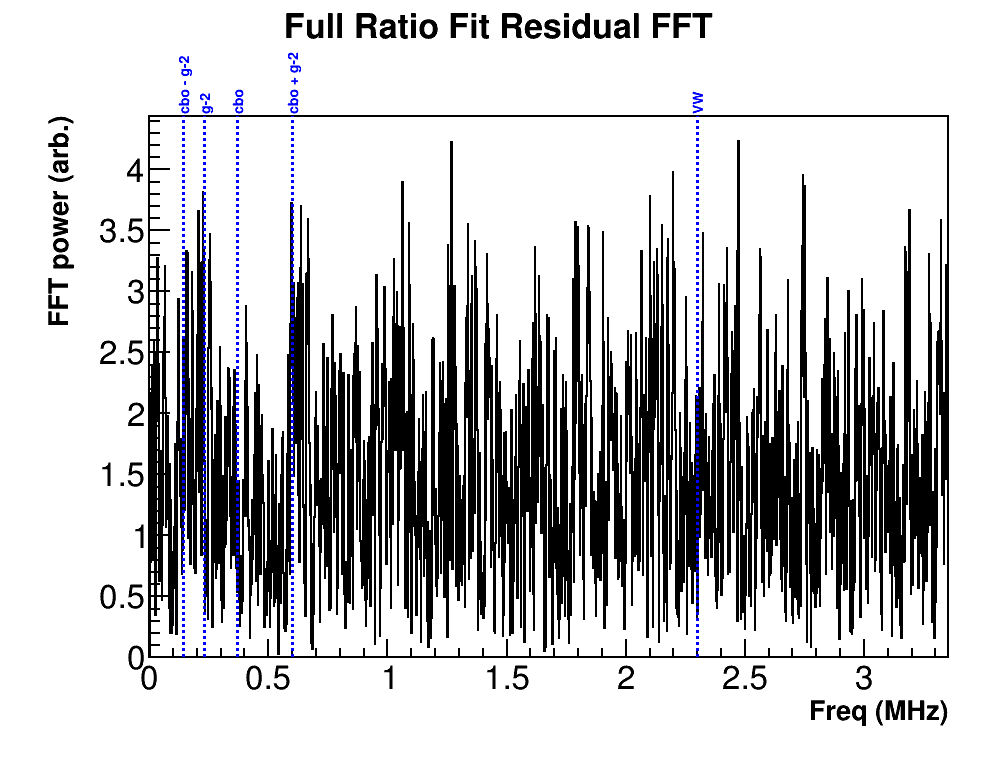
\includegraphics[width=\textwidth]{FFT_ratioCBOFit}
	    \caption[FFT_ratioCBOFit]{FFT of the residuals of the full ratio fit. No significant peaks remain in the ratio fit residuals after fitting with CBO terms. Overlayed are dotted lines for the \gmtwo, CBO, and vertical waist frequencies. Peaks close to the lines are coincidental but don't line up when zoomed in.}
	    \label{fig:FFT_ratioCBOFit}
	\end{figure}

	\begin{figure}[]
		\centering
		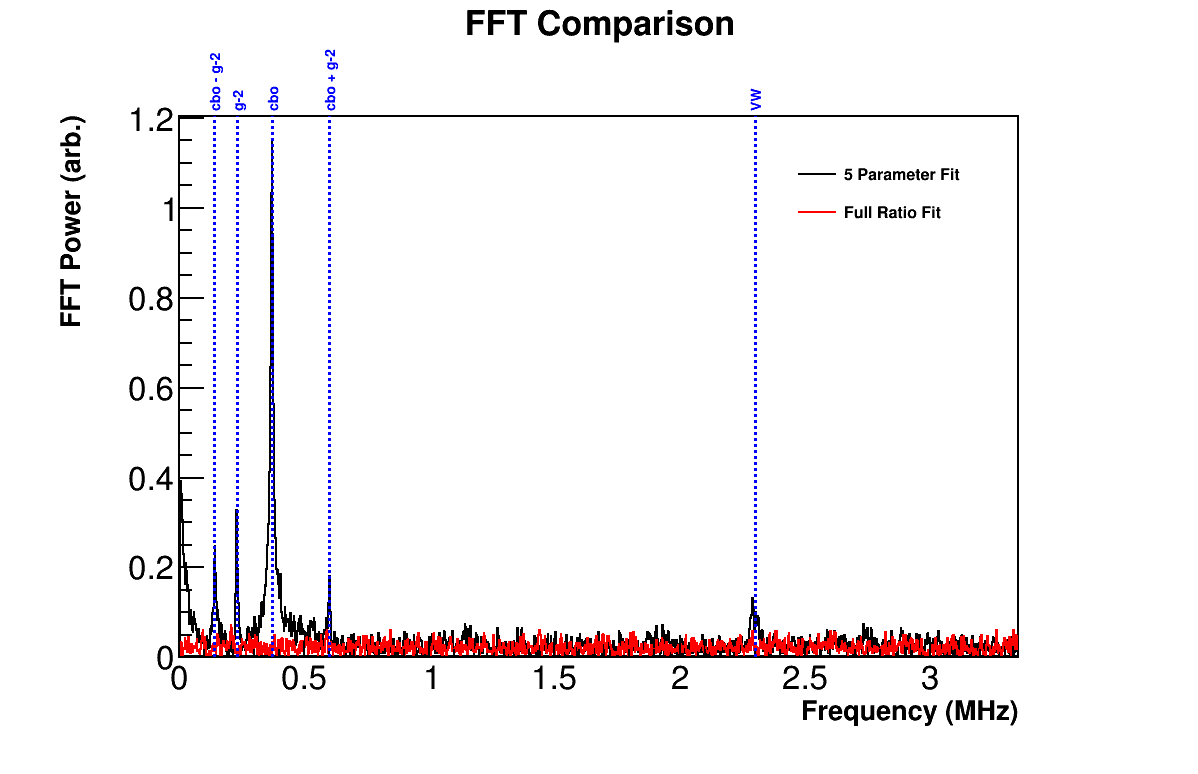
\includegraphics[width=\textwidth]{FFTComparison_RatioCBO}
	    \caption[FFTComparison_RatioCBO]{A plot of the FFT of the residuals of the fit for the five parameter fit compared to the ratio fit. In black is the FFT for a five parameter fit, where peaks for the CBO and vertical waist can be seen as well as the \gmtwo peak. In red is the FFT of the full ratio fit residuals, where it has been scaled up to be visible on this plot.}
	    \label{fig:FFTComparison_RatioCBO}
	\end{figure}

\clearpage

\section{Start time scans}

	Also necessary to determine whether the fit has been performed appropriately, is to perform start time scans. This procedure involves changing the start bound of the fit as a function of time, and making sure that fit results are consistent. If effects in the data are not properly accounted for, then fit parameters or the goodness-of-fit will change over time and will wander far outside the statistical limits defined by the reduction in data that is fitted. An example of this is shown in Section \ref{Sec:CBOFreq}, where the CBO freqency was originally modelled incorrectly. For the full ratio fit it turns out that this is the only effect that has a negative impact on the fit vs fit start time. As shown in Figure \ref{fig:Chi2FSScan} the goodness-of-fit is consistent over time, only wandering outside the statistical bands slightly. (This is also partly due to the randomization as mentioned in Section \ref{Sec:Randomization}.) Similarly Figure \ref{fig:FitStartScans} shows fit start time scans for each free parameter in the fit. All fit parameters lie comfortably within the statistical bands and are stable vs fit start time, indicating again that the fit is behaving properly.

	\begin{figure}[h]
		\centering
		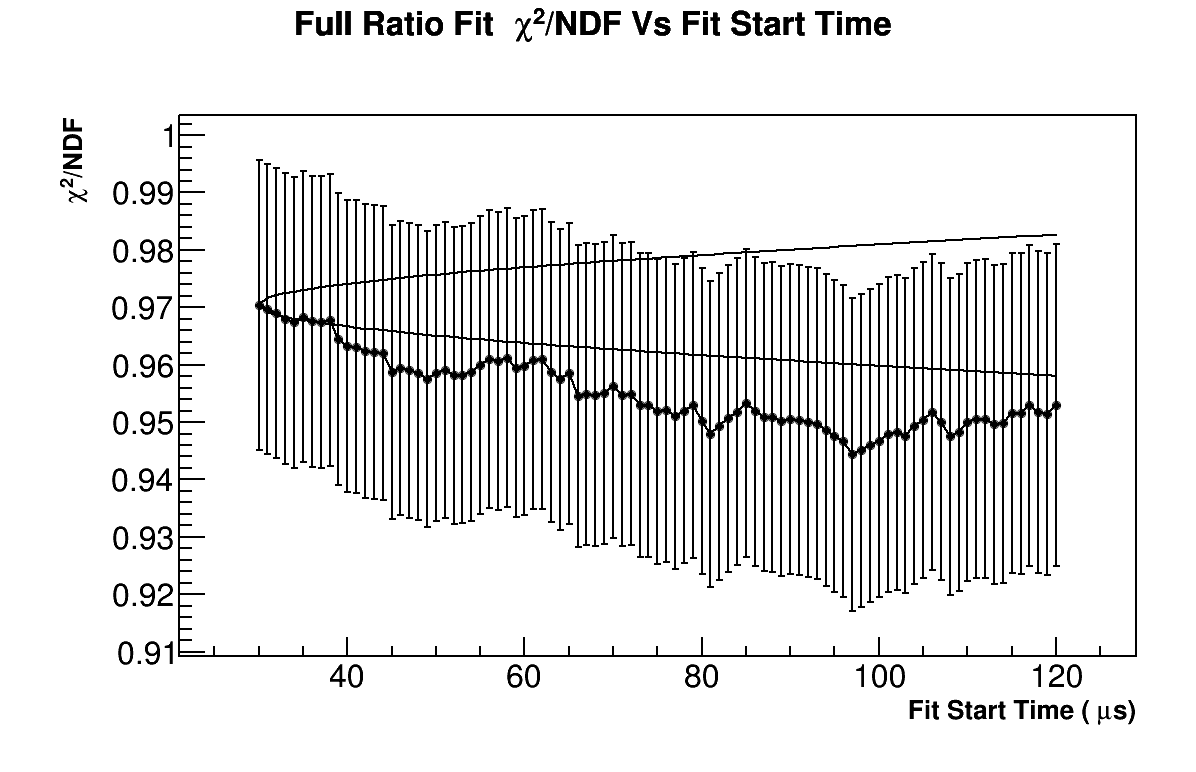
\includegraphics[width=\textwidth]{RatioCBO_Chi2NDF_Vs_FS_canv}
	    \caption[Chi2FSScan]{Plotted is the \chisq per degree of freedom vs the start time of the fit. The solid lines indicate the one sigma statistically allowed difference in the fit result coming from the reduction in the data included in the fit. The error bars on the points are calculated as $\sqrt{2/NDF}$.}
	    \label{fig:Chi2FSScan}
	\end{figure}


	\begin{figure}[]
	\centering
	    \begin{subfigure}[t]{0.45\textwidth}
		    \centering
			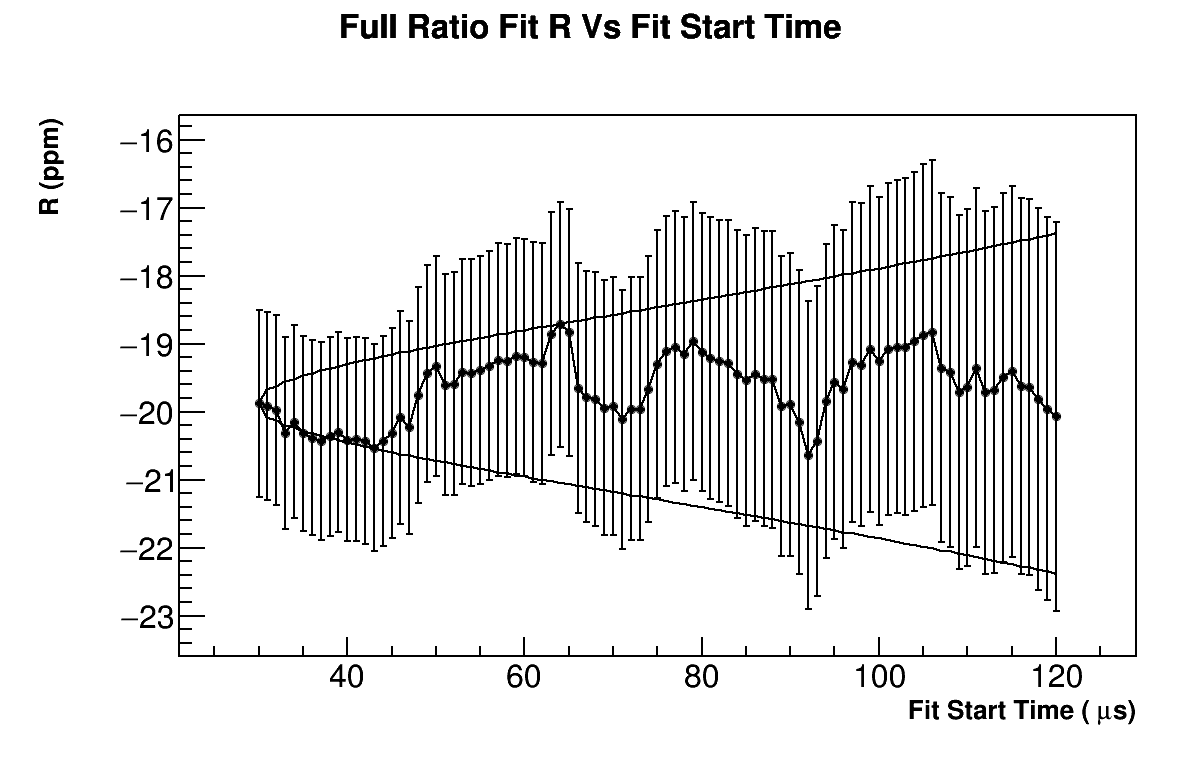
\includegraphics[width=\textwidth]{RatioCBO_R_FS_Canv}
		    \caption{Fitted R value vs fit start time.}
	    \end{subfigure}
	    \begin{subfigure}[t]{0.45\textwidth}
		    \centering
			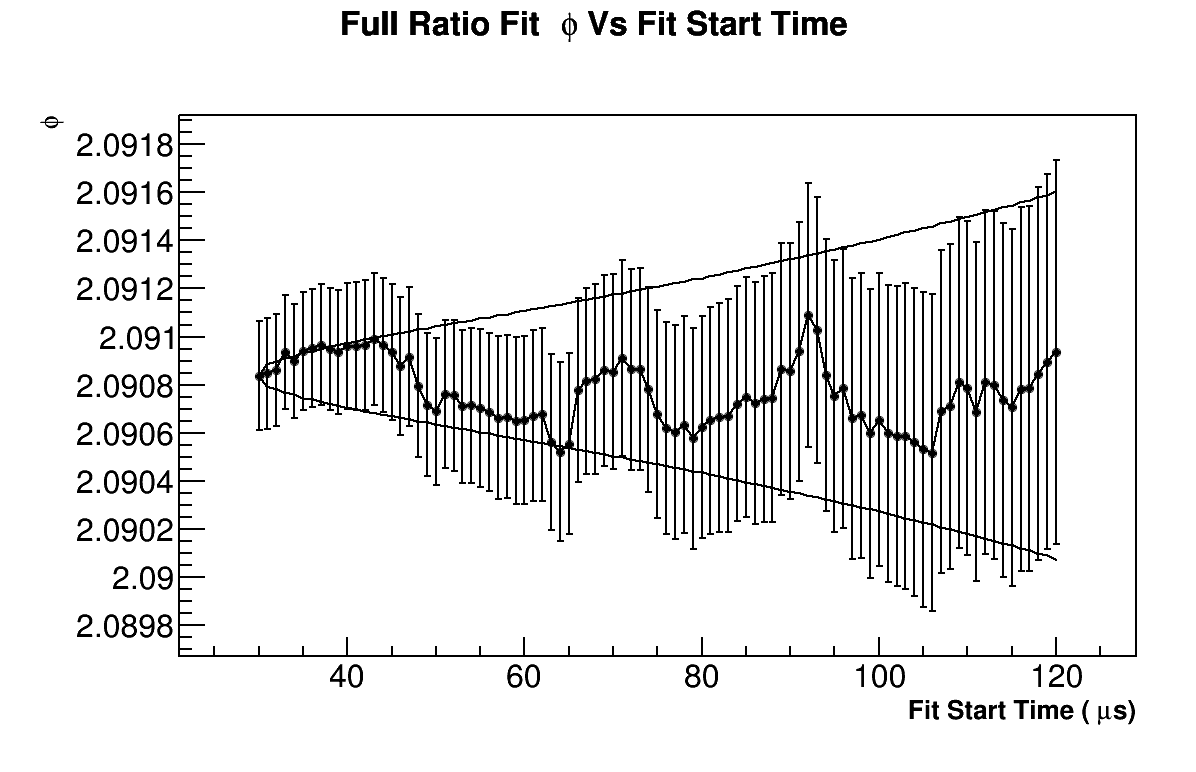
\includegraphics[width=\textwidth]{RatioCBO_phi_FS_Canv}
		    \caption{Fitted \gmtwo phase vs fit start time.}
	    \end{subfigure}% %you need this % here to add spacing between subfigures
	    \vspace{4mm}
	    \begin{subfigure}[t]{0.45\textwidth}
		    \centering
			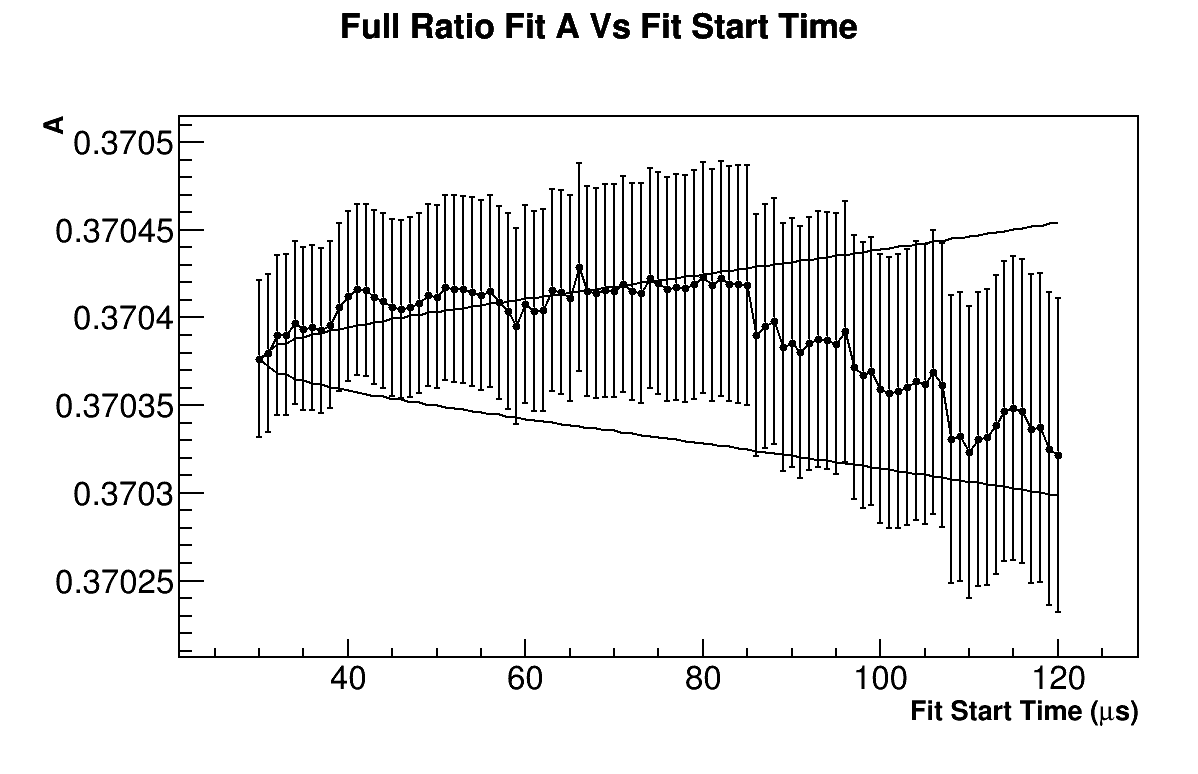
\includegraphics[width=\textwidth]{RatioCBO_A_FS_Canv}
		    \caption{Fitted asymmetry vs fit start time.}
	    \end{subfigure}
	    \begin{subfigure}[t]{0.45\textwidth}
		    \centering
			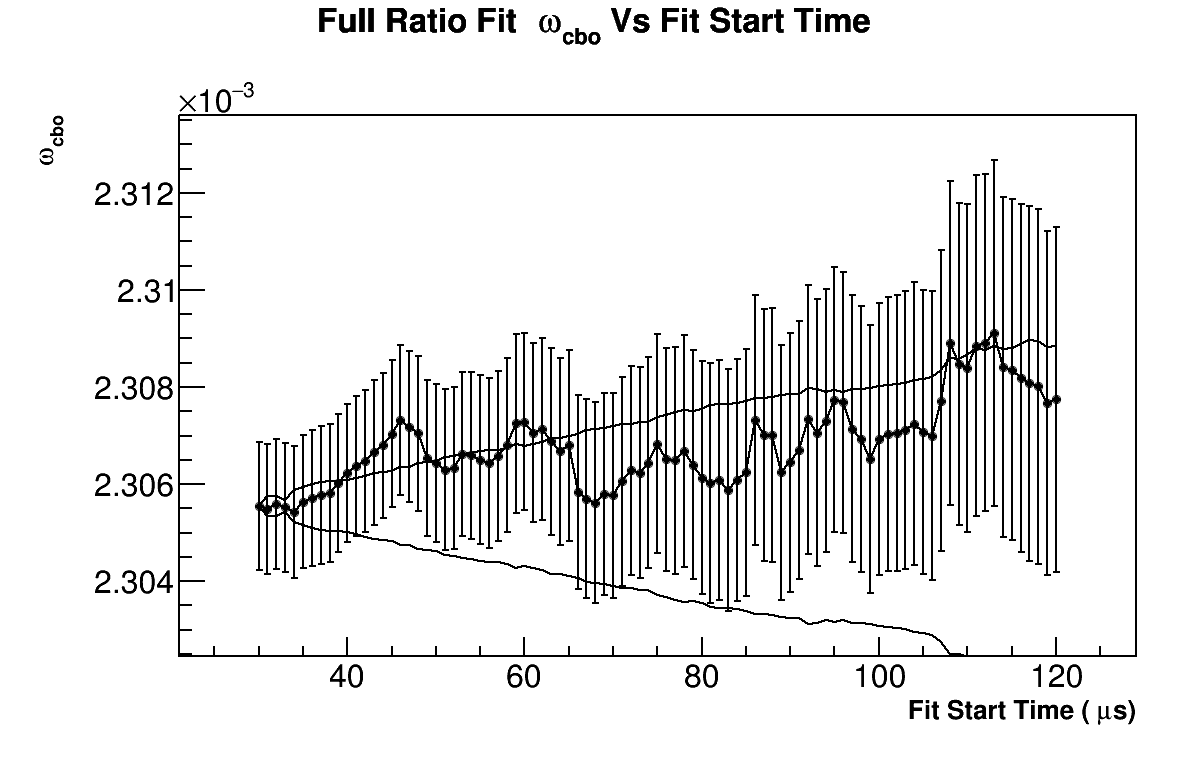
\includegraphics[width=\textwidth]{RatioCBO_omega_cbo_FS_Canv}
		    \caption{Fitted CBO frequency ($\omega_{0}$) vs fit start time.}
	    \end{subfigure}% %you need this % here to add spacing between subfigures
	    \vspace{4mm}
	    \begin{subfigure}[t]{0.45\textwidth}
		    \centering
			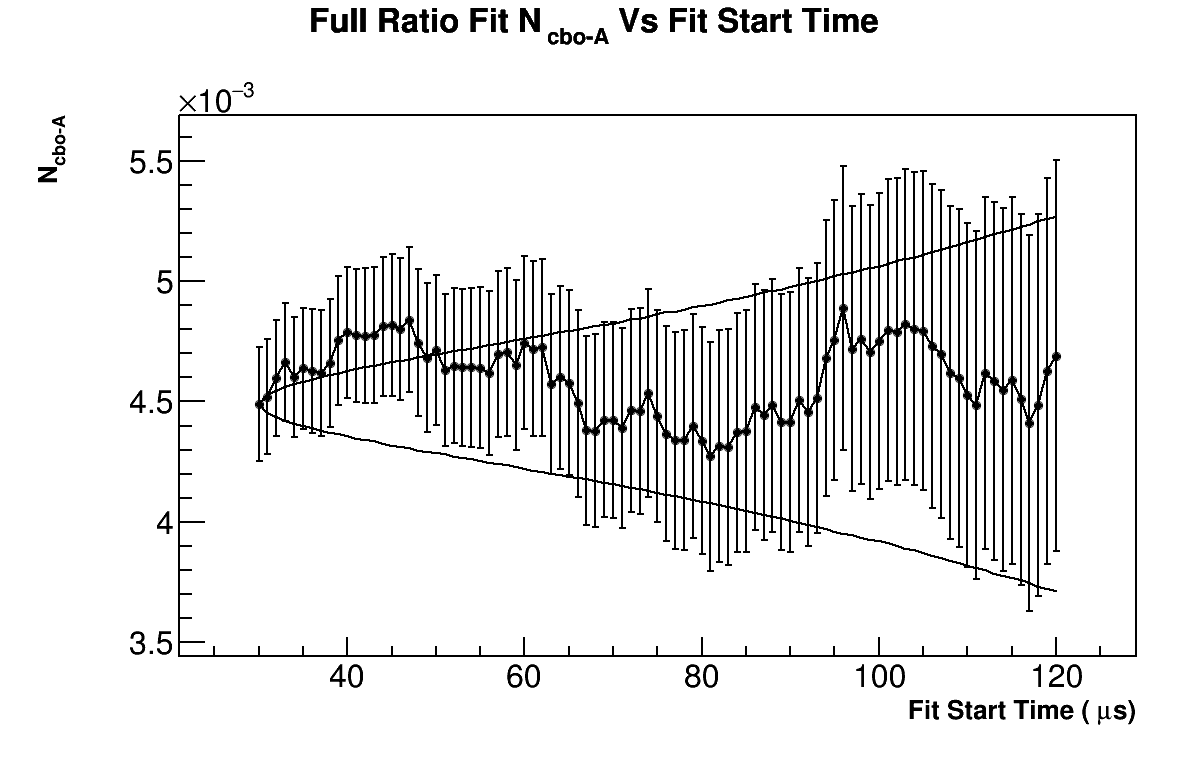
\includegraphics[width=\textwidth]{RatioCBO_N_cbo-A_FS_Canv}
		    \caption{Fitted CBO amplitdue vs fit start time.}
	    \end{subfigure}
	    \begin{subfigure}[t]{0.45\textwidth}
		    \centering
			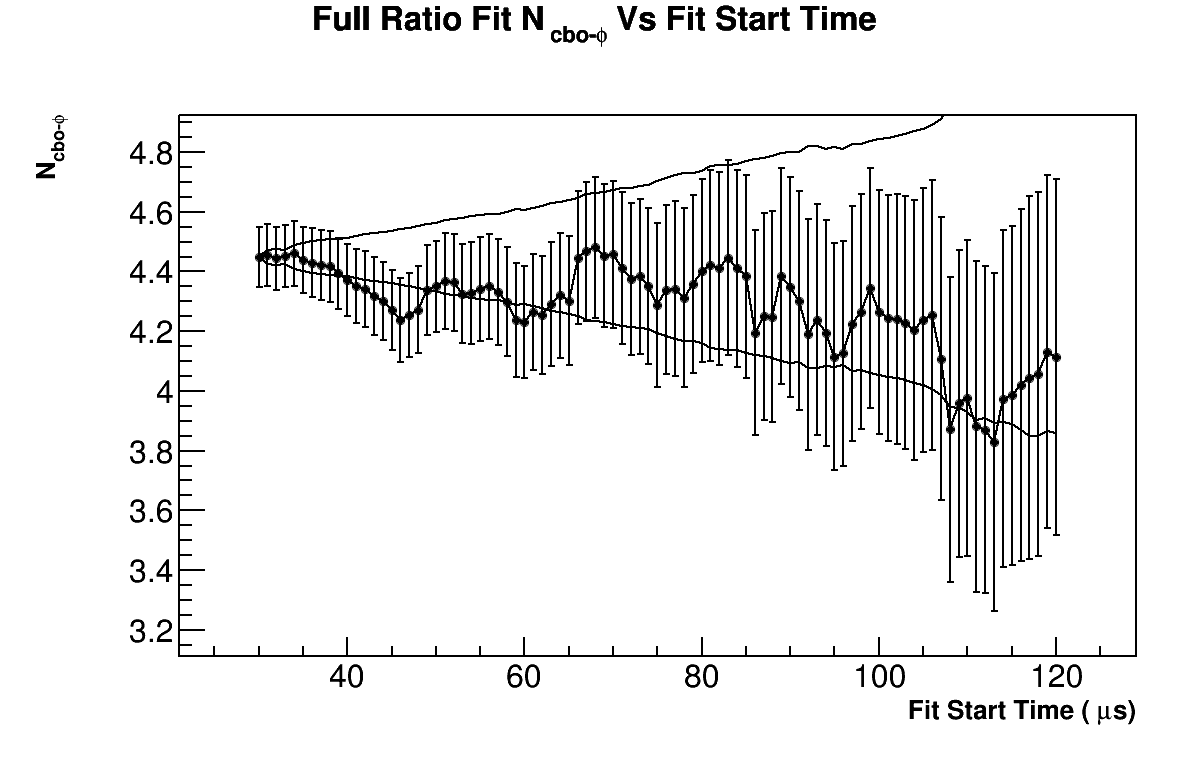
\includegraphics[width=\textwidth]{RatioCBO_N_cbo-phi_FS_Canv}
		    \caption{Fitted CBO phase vs fit start time.}
	    \end{subfigure}% %you need this % here to add spacing between subfigures
	\caption[FitStartScans]{Start time scans for the free parameters in the full ratio fit. All parameters are consistently within the one sigma statistical bands.}
	\label{fig:FitStartScans}
	\end{figure}


% \section{Stop time scans}

% I can produce stop time scans, and the results are consistent with the statistical significance bands, but some of the fits aren't perfect leading to some bad looking plots. Should I leave these out completely? Play more with the limits like I did to get the start time scans clean? Hack the plotting module to produce nicer looking plots? Or only include the good looking plots like R and the chi2?


\section{Results vs calorimeter}

	Finally results are examined on a per calorimeter basis. While there will be some differences in fit results due to the differing acceptance between the calorimeters, in general the results should be consistent.

	Still working on per calo fit stuff - will update plots and text when ready.

	\begin{figure}[h]
		\centering
		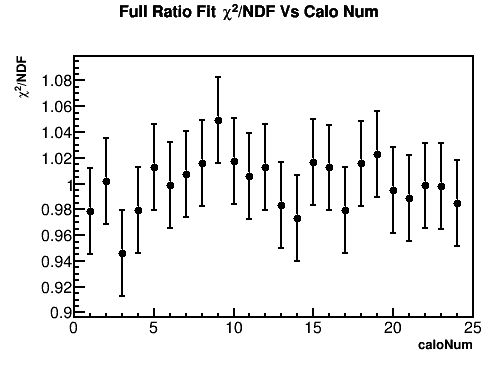
\includegraphics[width=.7\textwidth]{RatioCBOFit_Chi2NDF_Vs_Calo_Canv}
	    \caption[RatioCBOFit_Chi2NDF_Vs_Calo_Canv]{Plotted is the \chisq per degree of freedom vs calorimeter number.}
	    \label{fig:RatioCBOFit_Chi2NDF_Vs_Calo_Canv}
	\end{figure}


	\begin{figure}[h]
	\centering
	    \begin{subfigure}[t]{0.4\textwidth}
		    \centering
			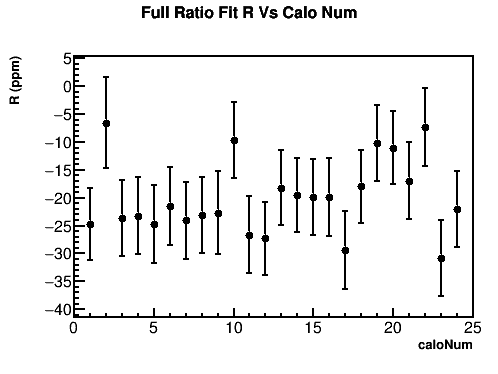
\includegraphics[width=\textwidth]{RatioCBOFit_R_Vs_Calo_Canv}
		    \caption{Fitted R value vs calorimeter number.}
	    \end{subfigure}
	    \hspace{4mm}
	    \begin{subfigure}[t]{0.4\textwidth}
		    \centering
			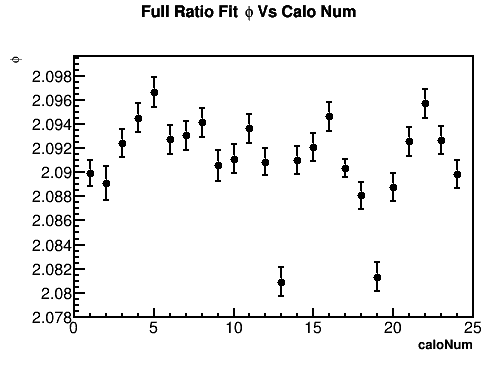
\includegraphics[width=\textwidth]{RatioCBOFit_phi_Vs_Calo_Canv}
		    \caption{Fitted \gmtwo phase vs calorimeter number. Calorimeters 13 and 19 lie behind the trackers leading to the different \gmtwo phases.}
	    \end{subfigure}% %you need this % here to add spacing between subfigures
	    \vspace{4mm}
	    \begin{subfigure}[t]{0.4\textwidth}
		    \centering
			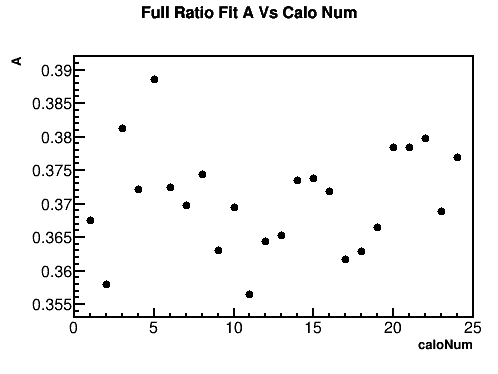
\includegraphics[width=\textwidth]{RatioCBOFit_A_Vs_Calo_Canv}
		    \caption{Fitted asymmetry vs calorimeter number.}
	    \end{subfigure}
	    \hspace{4mm}
	    \begin{subfigure}[t]{0.4\textwidth}
		    \centering
			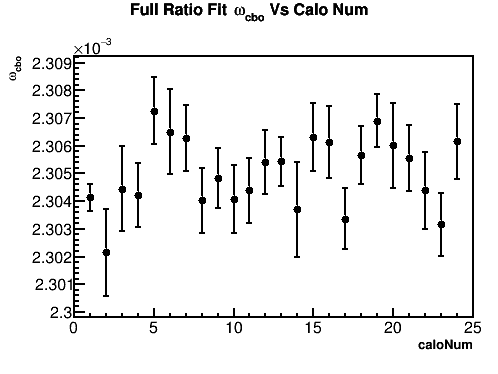
\includegraphics[width=\textwidth]{RatioCBOFit_omega_cbo_Vs_Calo_Canv}
		    \caption{Fitted CBO frequency ($\omega_{0}$) vs calorimeter number.}
	    \end{subfigure}% %you need this % here to add spacing between subfigures
	    \vspace{4mm}
	    \begin{subfigure}[t]{0.4\textwidth}
		    \centering
			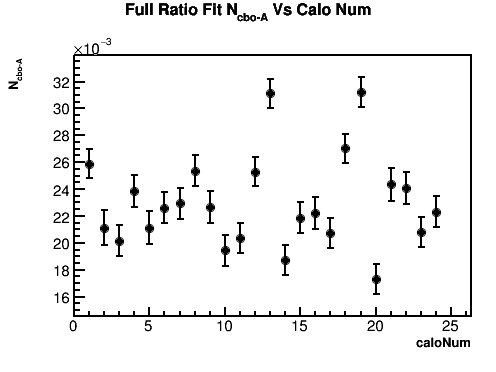
\includegraphics[width=\textwidth]{RatioCBOFit_N_cbo-A_Vs_Calo_Canv}
		    \caption{Fitted CBO amplitdue vs calorimeter number.}
	    \end{subfigure}
	    \hspace{4mm}
	    \begin{subfigure}[t]{0.4\textwidth}
		    \centering
			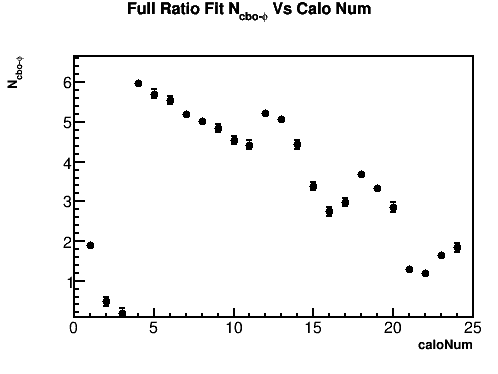
\includegraphics[width=\textwidth]{RatioCBOFit_N_cbo-phi_Vs_Calo_Canv}
		    \caption{Fitted CBO phase vs calorimeter number. The CBO phase varies from 0 to 2$\pi$ around the ring.}
	    \end{subfigure}% %you need this % here to add spacing between subfigures
	\caption[PerCaloPlots]{Full ratio fit parameter values vs calorimeter number.}
	\label{fig:PerCaloPlots}
	\end{figure}



